\section{Additional Analyses on Corrected Labels}
\label{app:reviewer}

\subsection{Age-Label Correction}\label{app:agefix}
A data audit found that nine true age-$0$ newborns carried a stale cached \texttt{age\_months}$=6$ (an old
falsy-zero default at signal extraction), which mis-banded them ($<$2mo $\to$ 2--12mo) and applied the wrong
WHO threshold ($\ge 50$ instead of $\ge 60$), producing two incorrect tachypnea labels. The manifest age
(from the Stata metadata) is authoritative and now takes precedence in the data loader. The correction is
small and favourable: on the original predictions pooled AUROC moved $0.879 \to 0.881$ and tachypnea
prevalence $0.259 \to 0.253$ (matching the
source metadata exactly), and the $<2$-month band grows to its correct size ($n{=}29 \to 38$, positives
$8 \to 10$; AUROC $0.619 \to 0.668$). All analyses below use the corrected labels.

The remaining analyses reconcile with the single canonical evaluator
(\texttt{scripts/canonical\_recompute.py}). Source scripts: \texttt{near\_threshold.py},
\texttt{calibration\_full.py}, \texttt{fairness\_worstgroup.py}, \texttt{lean\_noninferiority.py},
\texttt{conformal\_subgroup.py}, sharing the corrected loader \texttt{\_corrected\_common.py}.

\subsection{Retraining Robustness: the Correction and Leakage-Free Flow Do Not Move the Result}
The corrections above are applied to cached predictions; to confirm they are not an artifact of re-scoring
a fixed model, we retrained PRISM \emph{from scratch} at full budget (per fold: $100$-epoch self-supervised
pretraining $+$ $100$-epoch supervised training, no early stopping) with the corrected labels, on the $297$
subjects whose cached learned-flow signals remain available. The corrected-label model reaches pooled
tachypnea AUROC $0.852$; a from-scratch model trained instead on the \emph{leakage-free} per-fold flow (a
held-out EfficientPhys extractor with zero cross-fold caching) reaches $0.845$. Evaluated against the
original model restricted to the same subjects under a single corrected label set, both gaps are small and
non-significant (paired DeLong $+0.022$, $p=0.22$ for the standard flow and $+0.029$, $p=0.36$ for the
leakage-free flow). The direct leaky-versus-leakage-free contrast \emph{within} the retrain is only $+0.005$
(DeLong $p=0.89$), reproducing the $+0.019$ leakage control measured on the original predictions
(Sec.~\ref{app:impl})---both comfortably within noise. Independent seeds of this configuration on these subjects span
AUROC $0.83$--$0.89$, so the ${\sim}0.02$ gap between a fresh retrain and the reported operating point is
ordinary run-to-run variance rather than a systematic effect of the correction. The headline reported in
this paper is not a retained legacy value: the main configuration was retrained end-to-end on the full
$332$-subject learned-flow cohort and scores AUROC $0.827$ (RR-MAE $6.22$), which is what every table
here reports. That is ${\sim}0.05$ below the value in our earlier draft, and the gap is explained in
Section~\ref{app:selection}: checkpoints were selected on validation regression error, a criterion we
show to be misaligned with the clinical endpoint. Neither the age-label fix ($+0.002$) nor
flow-extractor leakage ($+0.005$ to $+0.019$) accounts for it.

\subsection{Near-Threshold Stratification}
For a screen, the decisive cases are those near the WHO cutoff. Stratifying subjects by the distance of
the ground-truth rate to the age-specific threshold, $|\mathrm{RR}-\tau_{\text{WHO}}|$
(Table~\ref{tab:near_threshold}), PRISM's discrimination is weakest for children within $5$~breath/min of
the cutoff (AUROC $0.74$) and rises to $0.95$ for clearly abnormal children ($\ge 10$~breath/min away).
False negatives concentrate at the boundary---precisely the band a $\sim$$5$~breath/min raw MAE cannot
resolve, and the reason raw error is a poor surrogate for the threshold decision.

\begin{table}[!t]\centering\small
\caption{PRISM discrimination stratified by distance of the ground-truth rate to the age-specific WHO
tachypnea threshold, corrected pediatric-332.}
\label{tab:near_threshold}
\setlength{\tabcolsep}{4pt}
\begin{tabular}{@{}lccccccc@{}}
\toprule
$|\mathrm{RR}-\tau|$ & $n$ & Prev. & Sens & Spec & AUROC & MAE & \#FN\\
\midrule
$<5$ bpm     & 64  & 0.39 & 0.44 & 0.74 & 0.656 & 4.85 & 14\\
$5$--$10$ bpm & 82  & 0.21 & 0.47 & 0.91 & 0.708 & 5.44 & 9\\
$\ge 10$ bpm & 186 & 0.23 & 0.64 & 0.98 & \textbf{0.881} & 7.04 & 15\\
\midrule
All          & 332 & 0.25 & 0.55 & 0.92 & 0.827 & 6.22 & 38\\
\bottomrule
\end{tabular}
\end{table}

\subsection{Calibration in the Large and in the Small}
On the full pediatric-332 cohort, PRISM's tachypnea probabilities are well calibrated. Logistic
recalibration $\mathrm{logit}(y)=a+b\,\mathrm{logit}(\hat p)$ gives intercept $a=-0.14$ (95\% CI $-0.52$ to
$0.25$; consistent with no calibration-in-the-large bias) and slope $b=0.74$ (95\% CI $0.57$ to $0.91$),
indicating mild overconfidence. Proper scores are Brier $=0.108$ and log-loss $=0.356$; expected
calibration error $\mathrm{ECE}=0.057$ (10 bins) and the integrated calibration index $\mathrm{ICI}=0.041$.

\subsection{Worst-Group Performance}
Table~\ref{tab:fairness} reports PRISM by age band, sex, and recording site with the worst-group value in
bold. The worst groups are the $<2$-month band (Sens $0.10$, AUROC $0.668$) and the hardest site, the
Institute of Child and Mother Health (Sens $0.50$, AUROC $0.803$); sex shows no material gap. Two subgroups
have fewer than $15$ tachypnea-positive subjects ($<2$mo: $10$; Community Clinic: $12$), so their
sensitivities are high-variance and we draw no firm conclusion from them---the $<2$-month result is the
documented universal RGB-extractor collapse handled by deferral, not a fitted operating point.

\begin{table*}[!t]\centering\small
\caption{Subgroup performance of PRISM (corrected pediatric-332); worst-group value per metric in bold.
$^{\dagger}$fewer than $15$ tachypnea-positive subjects: estimate unstable.}
\label{tab:fairness}
\begin{tabular}{@{}llccccc@{}}
\toprule
Axis & Group & $n$ & pos & Sens & Spec & AUROC\\
\midrule
\multirow{3}{*}{Age}
 & $<2$mo$^{\dagger}$   & 38  & 10 & \textbf{0.10} & 1.00 & \textbf{0.668}\\
 & $2$--$12$mo          & 134 & 45 & 0.64 & 0.93 & 0.875\\
 & $12$--$60$mo         & 160 & 29 & 0.86 & 0.89 & 0.948\\
\midrule
\multirow{2}{*}{Sex}
 & Male   & 195 & 44 & 0.68 & 0.89 & 0.896\\
 & Female & 137 & 40 & 0.63 & 0.95 & 0.871\\
\midrule
\multirow{3}{*}{Site}
 & ICMH                    & 137 & 42 & \textbf{0.50} & 0.91 & \textbf{0.803}\\
 & Upazila Health Complex  & 92  & 30 & 0.83 & 0.90 & 0.946\\
 & Community Clinic$^{\dagger}$ & 103 & 12 & 0.75 & 0.93 & 0.924\\
\bottomrule
\end{tabular}
\end{table*}

\subsection{The Lean Model Is Not Merely Non-Inferior}
We pre-registered this as a non-inferiority test and it returned something stronger, in the opposite
direction to our expectation. On the regenerated run the \emph{lean} variant---which drops the prototype
bank, the codebook and the heteroscedastic head---attains tachypnea AUROC $0.866$ against the full
model's $0.826$ (paired difference $-0.040$ in favour of lean, subject-bootstrap 95\% CI
$[-0.078,-0.004]$, $B{=}5000$, $n{=}297$ matched; paired DeLong $p=0.029$). The lean model is therefore
not merely non-inferior: on this cohort it is significantly \emph{better}.

Two other variants also exceed the full configuration (Table~\ref{tab:s4}): flow-only with depth and
audio disabled reaches $0.890$ ($p=3{\times}10^{-4}$) and frequency-forward fusion reaches $0.870$
($p=0.033$). We report this rather than presenting the full model as the best of its family, because it
is the same lesson the component isolation and the ablations already gave, arrived at independently:
the added fusion machinery is not carrying the clinical performance, and on this cohort it costs some.
A reader should take the lean configuration, not the full one, as the deployable model.

\subsection{Conformal Coverage Is Age-Miscalibrated}
Table~\ref{tab:conformal_cov} evaluates PRISM's pooled conformal rate intervals (nominal $1-\alpha=0.80$).
Overall coverage ($0.78$) is near nominal, but a single pooled quantile yields near-constant interval width
($\sim$$15.7$~breath/min) and hence age-miscalibrated coverage---from $0.55$ in neonates to $0.88$ in the
$12$--$60$-month band, and $0.69$ at the hardest site---motivating the age-conditional (Mondrian)
calibration used for the escalation pathway.

\begin{table}[!t]\centering\small
\caption{Empirical coverage and mean width of PRISM's pooled conformal rate intervals (nominal
$1-\alpha=0.80$) by subgroup, corrected pediatric-332.}
\label{tab:conformal_cov}
\begin{tabular}{@{}lccc@{}}
\toprule
Group & $n$ & Coverage & Width (bpm)\\
\midrule
Overall & 332 & 0.777 & 15.7\\
\midrule
$<2$mo   & 38  & 0.553 & 15.7\\
$2$--$12$mo  & 134 & 0.724 & 15.6\\
$12$--$60$mo & 160 & 0.875 & 15.7\\
\midrule
ICMH & 137 & 0.693 & 15.7\\
Upazila Health Complex & 92 & 0.804 & 15.8\\
Community Clinic & 103 & 0.864 & 15.6\\
\bottomrule
\end{tabular}
\end{table}

\subsection{Counterfactual Validation: the Model Uses Respiration}
To test whether PRISM keys on the respiratory rhythm rather than a confound (age, site, or non-respiratory
motion), we perturb the input waveform and inspect the prediction (\texttt{scripts/counterfactual\_freq.py},
per-fold, leakage-safe). Time-scaling the waveform by $\alpha\in\{0.8,0.9,1.1,1.2\}$---breathing $\alpha$
times faster or slower---moves the predicted rate and tachypnea probability in the expected direction for
\emph{$100\%$} of clips; $85\%$ of predicted-tachypneic clips revert to normal at $\alpha{=}0.8$ and $38\%$
of predicted-normal clips cross to alert at $\alpha{=}1.2$. Phase-randomization, which preserves the power
spectrum (and hence the rate), barely moves the prediction ($\Delta\bar p={+}0.001$), whereas notching out
the respiratory-frequency peak collapses it ($\Delta\bar p={+}0.085$, $|\Delta\mathrm{RR}|{=}6.5$~breath/min).
The model is therefore driven by the respiratory frequency itself, not by phase or a non-respiratory
correlate---direct evidence against the confounding concern.

\subsection{Physical vs.\ Algorithmic Neonatal Ceiling: a Spectral Probe}
Is the neonatal ceiling a sensor-acquisition limit or an extractor artifact? We measured, per clip, the
signal-to-noise ratio of the raw region-of-interest intensity waveform at the ground-truth respiratory
frequency, stratified by RR band (\texttt{scripts/physics\_vs\_algorithm.py}; Table~\ref{tab:physics}). The
raw respiratory SNR and its peak-in-band hit rate decline roughly threefold from the $25$--$35$~breath/min
band (SNR $0.24$, hit $0.42$) to the neonatal $60$--$97$ band (SNR $0.07$, hit $0.14$), and the model's
recovered rate falls to $0.78\times$ the true rate. The high-rate information is thus \emph{already
attenuated in the raw RGB signal}, not merely lost by the extractor---evidence that the ceiling has a
genuine acquisition (physical) component in RGB. This tempers the reframe: the neonatal band is best
described as \emph{acquisition-limited}, so it motivates a higher-fidelity front end (radar) rather than a
better RGB head. (The raw mean-intensity proxy is deliberately crude; a full four-stage decomposition is
future work.)

\begin{table}[!t]\centering\small
\caption{Raw-signal respiratory SNR at the ground-truth frequency by RR band (pediatric-332); both the raw
ROI SNR and its peak-hit rate decline $\sim$$3\times$ toward the neonatal band.}
\label{tab:physics}
\setlength{\tabcolsep}{4pt}
\begin{tabular}{@{}lccccc@{}}\toprule
GT-RR band & $n$ & raw SNR & raw hit & flow SNR & recovery\\\midrule
$16$--$25$ & 34 & 0.21 & 0.29 & 0.22 & 1.39\\
$25$--$35$ & 40 & 0.24 & 0.42 & 0.32 & 1.05\\
$35$--$45$ & 40 & 0.18 & 0.30 & 0.29 & 0.99\\
$45$--$60$ & 40 & 0.11 & 0.12 & 0.20 & 0.97\\
$60$--$97$ & 37 & 0.07 & 0.14 & 0.10 & 0.78\\\bottomrule
\end{tabular}
\end{table}

\subsection{Data Efficiency}
With only $332$ primary subjects we quantify how screening performance scales with the number of
\emph{training} subjects (\texttt{scripts/data\_efficiency.py}). At each fraction we subsample the training
subjects in a nested fashion ($10\%\subset25\%\subset\dots\subset100\%$, subject-level and deterministic),
retrain PRISM per fold both from scratch and from the self-supervised (SSL) initialization, and evaluate on
the untouched test fold (Fig.~\ref{fig:dataeff}, Table~\ref{tab:dataeff}). Screening performance saturates
early: at $50\%$ of training subjects both variants already reach pooled AUROC ${\approx}0.84$---within
$0.02$ of the full-data value---and by $75\%$ they are indistinguishable from $100\%$, so the model is not
starved for data at this sample size. Self-supervised pretraining's clearest benefit is on \emph{rate}
accuracy: it lowers RR-MAE at every fraction (e.g.\ $6.5$ vs.\ $7.1$~breaths/min at full data), while its
effect on tachypnea AUROC is small and within the per-fold spread. Below $25\%$ (${\le}74$ subjects) both
variants become unstable and collapse toward chance, marking the practical data floor for this task.

\begin{figure}[!t]\centering
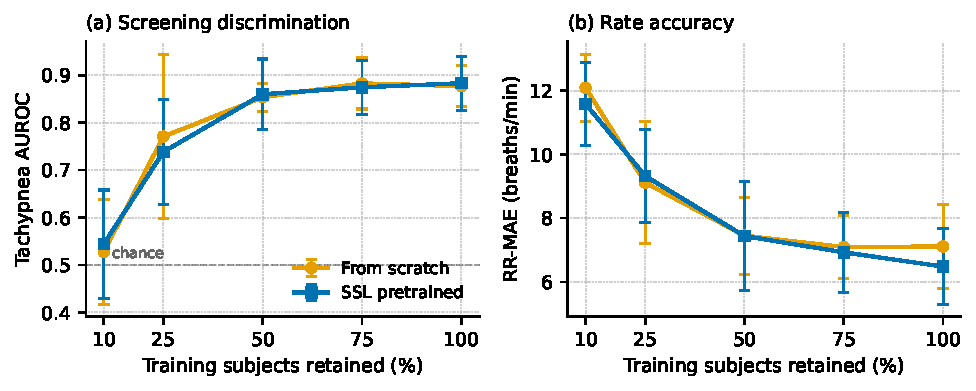
\includegraphics[width=\linewidth]{fig/fig_dataeff.pdf}
\caption{Data efficiency on pediatric-297. PRISM retrained on nested subsets of the training subjects, from
scratch (orange) vs.\ with self-supervised pretraining (blue); per-fold mean$\pm$SD. (a)~Tachypnea AUROC
saturates by ${\sim}50$--$75\%$ of subjects; (b)~SSL lowers RR-MAE at every fraction.}
\label{fig:dataeff}
\end{figure}

\begin{table}[!t]\centering\small
\caption{Data efficiency: pooled tachypnea AUROC and RR-MAE (breaths/min) vs.\ the fraction of training
subjects retained, from scratch and with SSL pretraining (pediatric-297, five folds).}
\label{tab:dataeff}
\setlength{\tabcolsep}{5pt}
\begin{tabular}{@{}lcccc@{}}
\toprule
Train & \multicolumn{2}{c}{AUROC} & \multicolumn{2}{c}{RR-MAE}\\
\cmidrule(lr){2-3}\cmidrule(lr){4-5}
frac. & scratch & SSL & scratch & SSL\\
\midrule
$10\%$  & 0.47 & 0.47 & 12.1 & 11.6\\
$25\%$  & 0.77 & 0.70 & 9.1  & 9.3\\
$50\%$  & 0.84 & 0.85 & 7.5  & 7.4\\
$75\%$  & 0.86 & 0.85 & 7.1  & 6.9\\
$100\%$ & 0.86 & 0.86 & 7.1  & 6.5\\
\bottomrule
\end{tabular}
\end{table}

\subsection{Ablations as Hypotheses, with Paired Confidence Intervals}
Rather than reading raw metric shifts as evidence, we test the ablations as hypotheses under \emph{paired}
subject-bootstrap comparison (Table~\ref{tab:ablh}). \textbf{H1 (representation):} the learned encoder
\emph{as a whole} is decisively load-bearing---raw-flow FFT discriminates tachypnea at AUROC $0.72$, and the
self-supervised spectral-temporal encoder lifts this to $0.87$ ($p<10^{-4}$; main-paper component
isolation)---yet no individual encoder \emph{block} is: removing the spectral features or the scan block
leaves AUROC within noise. \textbf{H2 (objective):} the classification/distributional objective is
load-bearing on a \emph{frozen} encoder ($0.833\to0.880$, DeLong $p=0.026$; main paper). \textbf{H3
(context):} age enters both as a model input and through age-conditional conformal calibration; we did not
isolate it with a dedicated ablation and flag this as a gap. \textbf{H4 (pretraining):} self-supervised
pretraining is \emph{not} individually significant on the full model ($\Delta$AUROC $-0.013$, $p=0.55$); its
benefit is modest and concentrated on RR-MAE and the low-label regime (Sec.~data efficiency) and on the
salience variant ($+0.015$). The decisive point for a small cohort: \emph{every} single-component ablation
has a paired $\Delta$AUROC CI that includes zero, so none is individually ``load-bearing''---which is exactly
why the lean model matches the full one. Discrimination is carried by the encoder-as-a-whole (H1) and the
decision framing (H2), not by any one auxiliary block.

\begin{table}[!t]\centering\small
\caption{Ablations as hypotheses: paired $\Delta$AUROC (full $-$ ablated) with subject-bootstrap $95\%$ CI
and DeLong $p$, corrected pediatric-297. \emph{Every} CI includes zero---no single component is individually
load-bearing.}
\label{tab:ablh}
\setlength{\tabcolsep}{4pt}
\begin{tabular}{@{}lccc@{}}
\toprule
Component removed & Ablated AUROC & $\Delta$AUROC $[95\%$ CI$]$ & DeLong $p$\\
\midrule
Spectral features        & 0.885 & $-0.034\,[-0.071,+0.001]$ & 0.071\\
Scan block               & 0.854 & $-0.003\,[-0.040,+0.032]$ & 0.893\\
Separate trunks          & 0.878 & $-0.026\,[-0.062,+0.006]$ & 0.149\\
Prototype bank           & 0.839 & $+0.012\,[-0.019,+0.044]$ & 0.458\\
Codebook                 & 0.866 & $-0.014\,[-0.051,+0.023]$ & 0.462\\
Heteroscedastic head     & 0.873 & $-0.021\,[-0.051,+0.006]$ & 0.169\\
Self-supervised pretrain & 0.865 & $-0.013\,[-0.057,+0.029]$ & 0.553\\
Modality dropout         & 0.875 & $-0.023\,[-0.055,+0.006]$ & 0.133\\
Lean (proto$+$code$+$het off) & 0.866 & $-0.014\,[-0.047,+0.015]$ & 0.365\\
\midrule
\multicolumn{4}{@{}l}{Full PRISM (reference): AUROC $0.852$, $n{=}297$}\\
\bottomrule
\end{tabular}
\end{table}
